\section{Method}
\label{sec:method}
This section is organized around three key questions in the context of ML license analysis: (i) How to determine the corresponding conditions in licenses for certain model reuse mechanisms? (ii) How to capture the dependency structure of a machine learning project? (iii) What types of non-compliance exist in ML projects and how to assess them?
We will present our solutions to these questions in the following sections.

\subsection{Taxonomy for ML License Analysis}
Determining the corresponding conditions in licenses is a challenging task for ML projects due to the conceptual ambiguities in existing licensing language and the disorganization in current ML licensing practices.
For example, CC-BY-ND prohibits the sharing of derivatives of licensed materials.
However, its definition of making derivatives is unclear in the context of ML domain.
For instance, should embeddings of a corpus be considered a derivative work upon that corpus?
Unfortunately, even though Creative Commons provides a flow chart to illustrate the trigger conditions of CC licenses in the context of AI activity~\cite{creative2023artificial}, it raises another question: \textit{Is the output considered protectable copyright subject matter?}
The answer depends on how the embedding activity is interpreted, for example, considering it as a translation of the original work can trigger the CC license.

MDL advocates the use of a \textit{Top Sheet} to delineate what ML activities are allowed with data~\cite{benjamin2019towards}, but this proposal is rarely implemented in practice (life would be easier if it were widely accepted). 
Making things more complex, some projects release their models under free content licenses, like LayoutLMv3 model~\cite{huang2022layoutlmv3}, which is licensed under CC-BY-NC-SA-4.0. 
This disorganization makes it unclear what kinds of ML activities can trigger licenses conditions in different contexts.
An ideal and elegant solution would be to encourage licensors to make context-appropriate adaptations in their license agreements or terms of use to clarify the granted rights related to ML activities. 
However, some ML components may be composed of prior works that are shared under copyleft license templates, which may disallow such relicensing of their derivatives to a new license.
Therefore, it is necessary to establish practical rules to bridge AI activities and existing licensing language.

To address the above challenge, we propose a result-based taxonomy that categorizes all AI activities into four categories based on the forms of their results. 
In our taxonomy, there are four categories of AI activities: Combination, Amalgamation, Distillation, and Generation, which are defined by four forms of their results, respectively: 1) Combination with strong separation; 2) Combination with weak separation; 3) Derivatives from concepts; and 4) Derivatives from data.
Correspondingly, we can also categorize the usage behaviors in licensing language into these four categories based on their outcome forms.

We leverage Figure~\ref{fig:tax} to illustrate this idea.
The left side consists of a list of AI activities, many of which pertain to model reusing methods, categorized based on the forms of their results.
The middle part is our taxonomy that can classify these AI activities.
Following this rule, we can also identify the corresponding terms in natural language license text shown on the right side.
For example, Mixture of Experts (MoE) leverages a gating network to ensemble a batch of weak learners~\cite{jacobs1991adaptive}, which leads to a combination with strong separation and aligns with licensing terms like link, portion, collection, etc.
Unlike combination, the results of amalgamation are difficult (or impossible) to separate, corresponding to AI activities such as modification, fine-tuning, model fusion, etc~\footnote{Whether embeddings constitute a combination with weak separation depends on the specific case. In ModelGo, we classify embeddings as amalgamation if they are created under a content license that treats translation as a form of modification.}. 
These unrecoverable revision of original works are corresponding license text like adapt, alter, remix, etc.
Distillation and generation are derivatives of original works, which means the results will not contain any portion of the original works. 
These two AI activities are mostly defined in AI model licenses but are not covered by traditional OSS licenses and free content licenses.

By now, we can ascertain the suitable permissions, limitations, and responsibilities for each AI activity based on the license language, even when the license type is not an exact match.
However, its necessarily to emphasize three points.
First, our proposed method only applies in cases where ambiguities exist in the definition. 
If the conditions of certain AI activities are explicitly defined in the license, then we should directly follow that.
Second, due to the various definitions adopted in different licenses, the bridging rules depend on each specific case and may differ from Figure~\ref{fig:tax}.
Lastly, one AI activity may trigger multiple license conditions. For example, a fine-tuned model can be seen as a combination with weak separation of the original model, while it can also be viewed as a derivative from fine-tuning data.
Therefore, we should design a mechanism to trace these multi-source dependency structures in ML projects, which we will detail in the next section.
 
\begin{figure}[t]
    \centering
    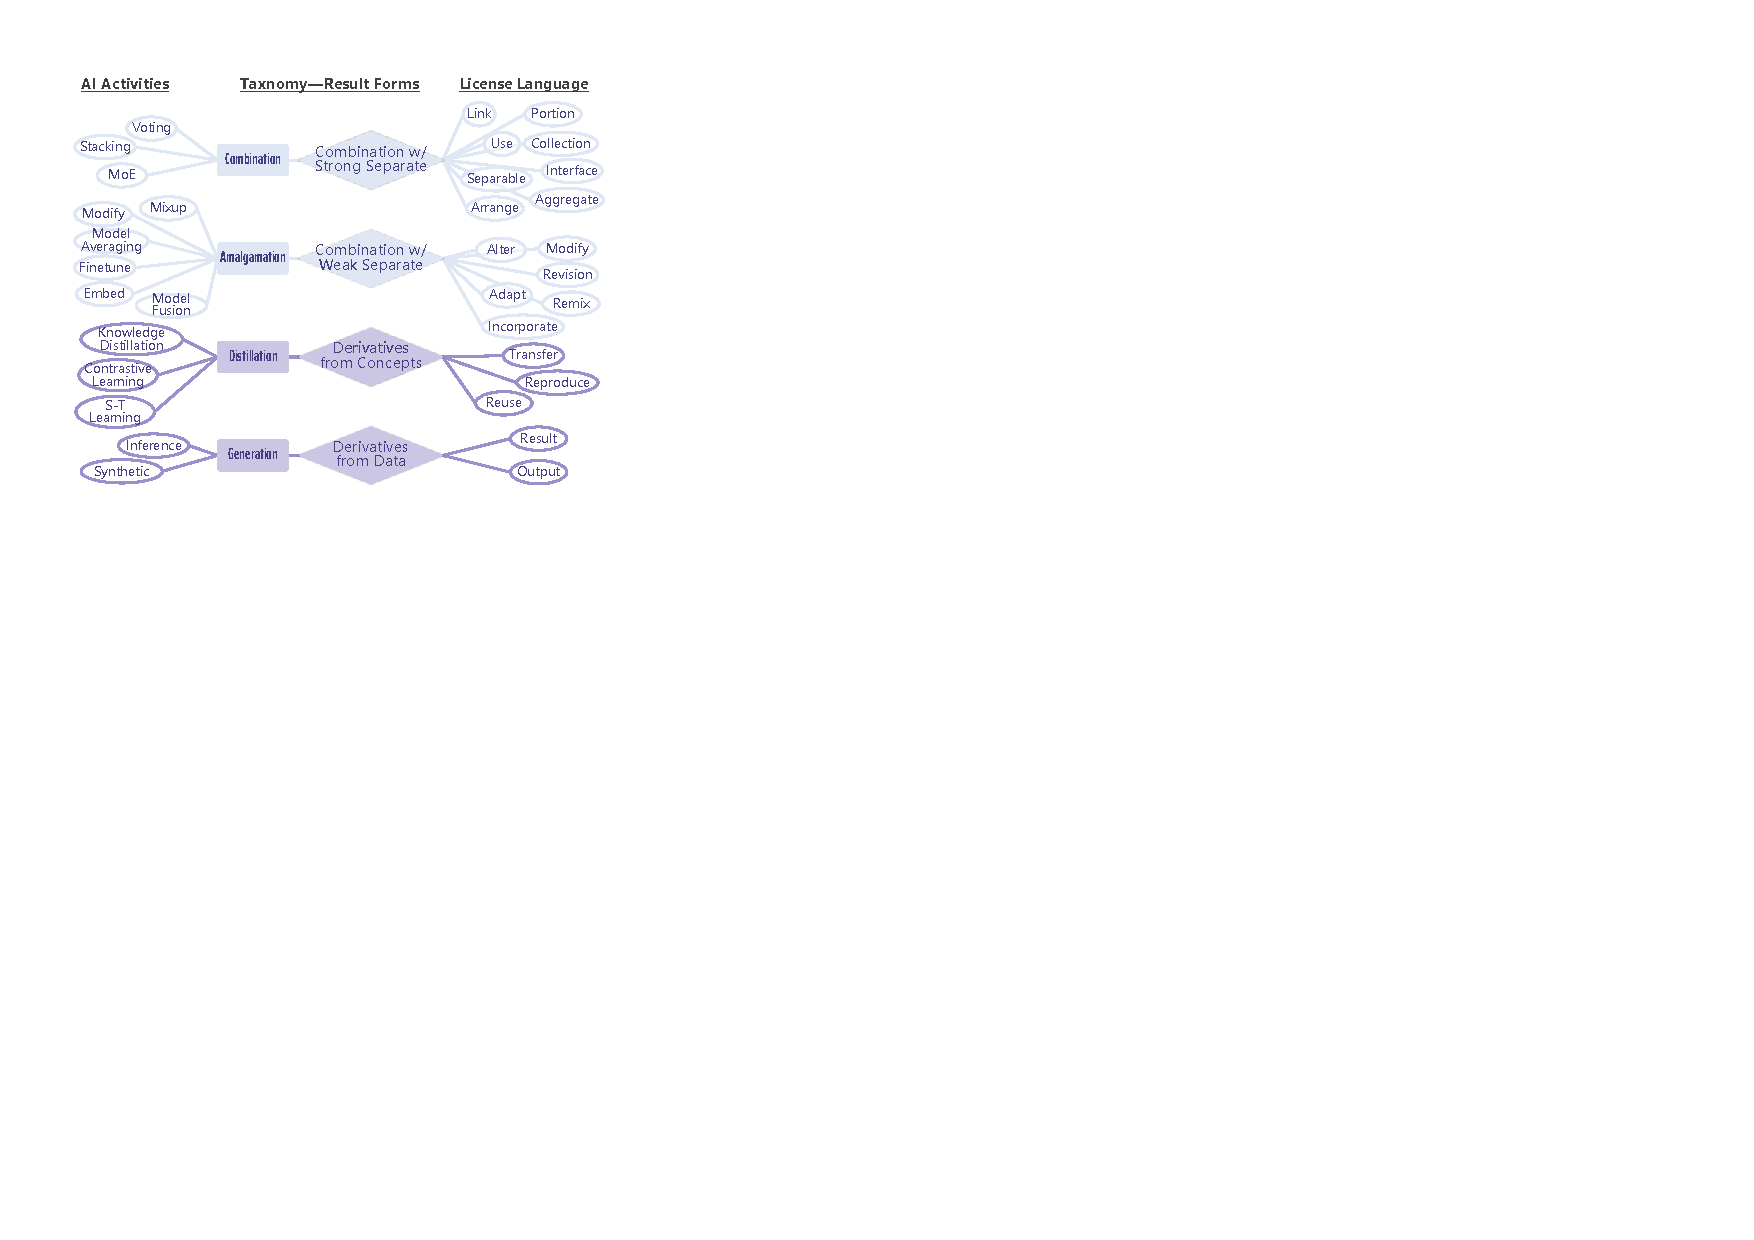
\includegraphics[width=\linewidth]{fig/taxonomy.pdf}
    \caption{Our proposed taxonomy bridging AI activities and license terms based on their result forms.}
    \Description{}
    \label{fig:tax}
    \vspace{-5mm}
\end{figure}

%translated, altered, arranged, transformed, or otherwise modified 
%Licensing Language Requires Standardization and  to ML and AI
%the notion of derivative work is ill defined
%conceptual ambiguities in existing licensing language
%There is no consensus on whether the use

\subsection{Structure of ML Projects}
ML projects have unique dependency relationships compared to OSS projects, like the dependencies between generated content and generation model, as well as between training data and trained model.
We can summarize these dependencies in ML projects into three categories:
\begin{itemize}[leftmargin=*]
    \item \textbf{Mix-works} be embeded in the new work, either verbatim or in part, in a tangible form.
    They usually result from direct copying of original components or reusing them through AI activities like combination and amalgamation. These components are embedded into ML projects and must be released with the new work. 
    For example, if we release a new work utilizing Mixture of Experts (MoE), it is equivalent to releasing all weak learners.

    \item \textbf{Sub-works} are similar to mix-works, but the difference is that they are not embedded in the new work. For instance, if we manage to release MoE model along with the data used for training the gating network, then this data will be regarded as the sub-works of MoE model.
    
    \item \textbf{Aux-works} are components used to build the new work and are either included in it or released with it. For example, the original model used for knowledge distillation.
\end{itemize}

Figure~\ref{fig:stru} illustrates the structure of a work constructed by reusing multiple components in the context of ML projects.
The final ML project may be constructed through iterative reuse of other works, resulting in a ternary dependencies tree for this project.
The reason we need this specially-designed tree structure is that works with different dependency types have different license condition proliferation rules, which need to be handled separately during subsequent license analysis. 


\begin{figure}[t]
    \centering
    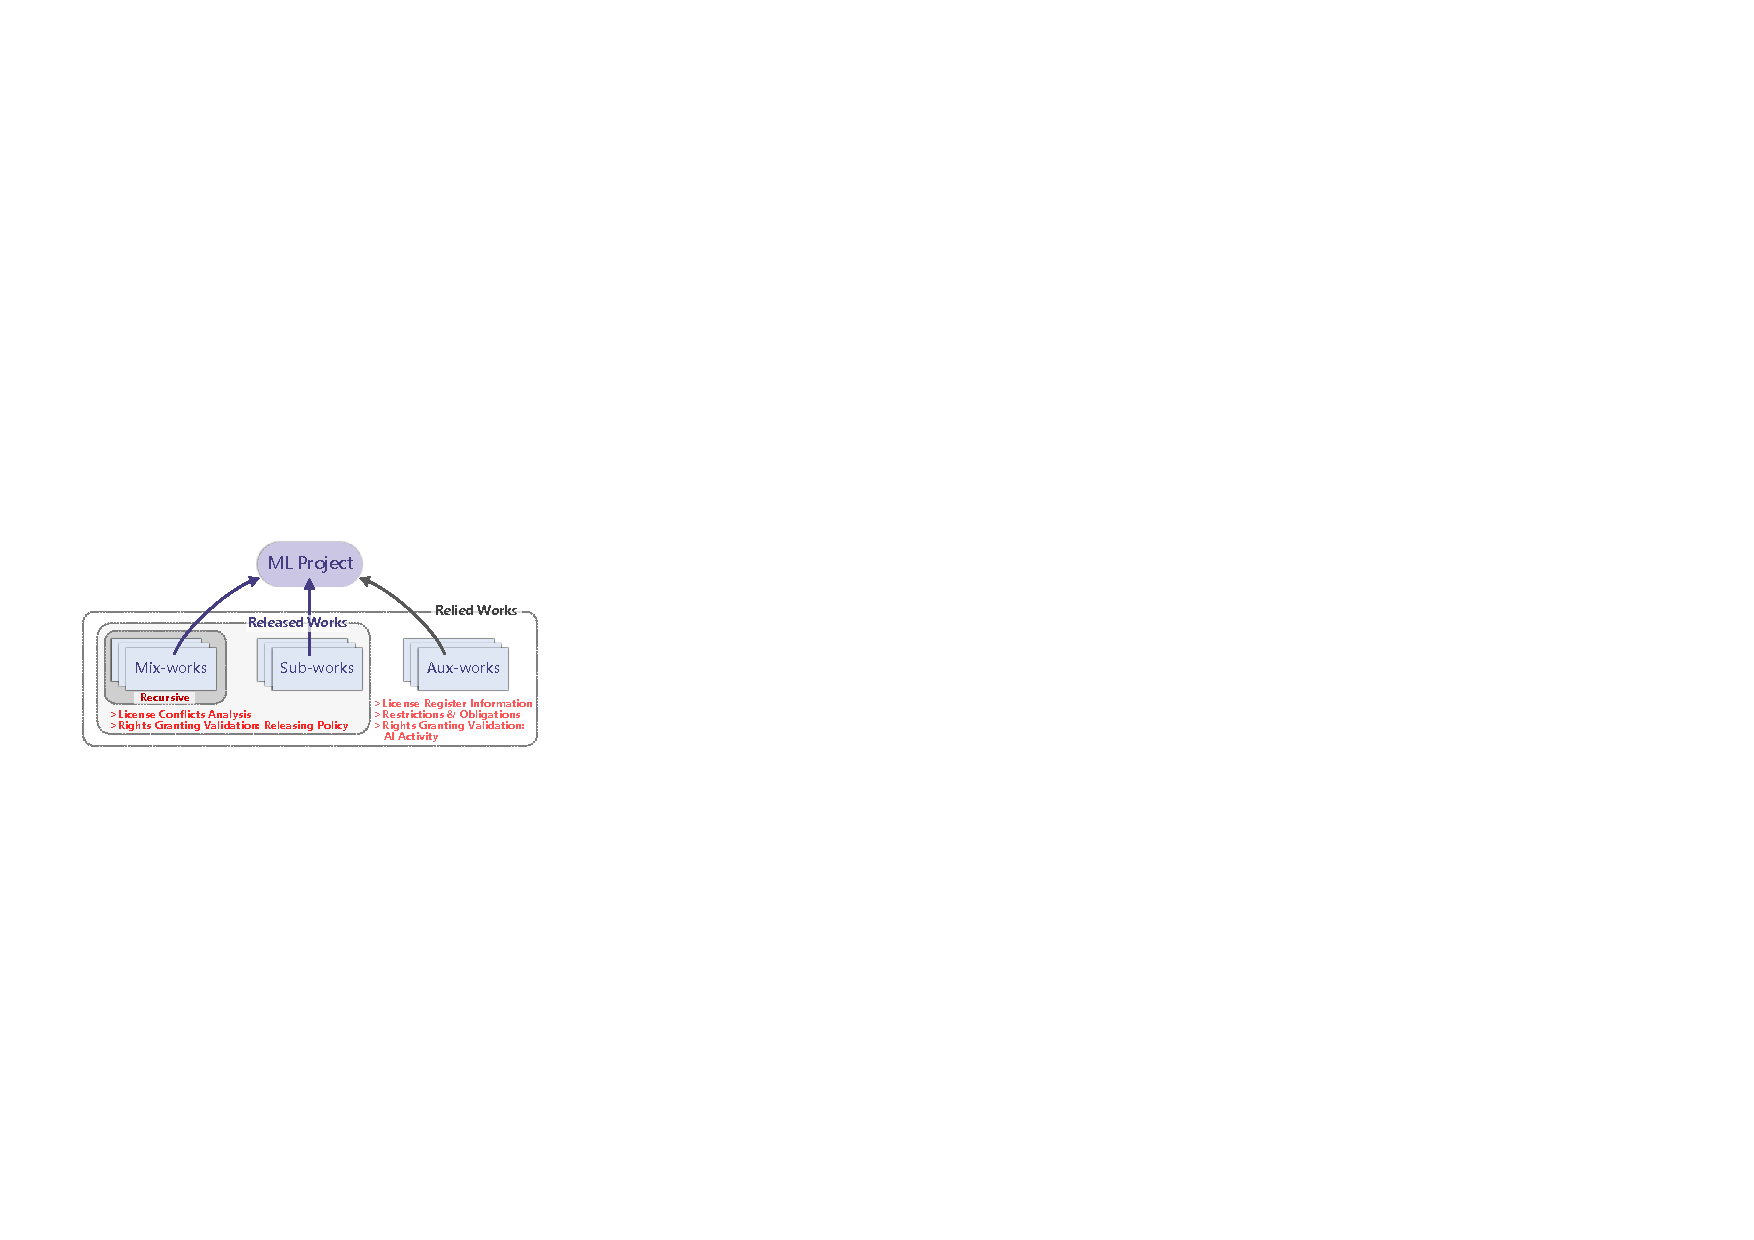
\includegraphics[width=\linewidth]{fig/structure.pdf}
    \caption{The proposed structure for capturing work dependencies in the context of ML projects with multiple reused components.}
    \Description{}
    \label{fig:stru}
    \vspace{-5mm}
\end{figure}

\subsection{License Analysis in ML Projects}

We have outlined all the necessary preparation steps for license analysis in previous sections.
Their detailed implementations in ModelGo are as follows.

\textbf{Preparation Step 1}: Following our proposed taxonomy, we have manually transcribed the terms in the license text to a standard machine-readable file in YAML format~\footnote{We attempted to use chatGPT to generate this content, but it often behaved unreliably in understanding our taxonomy and produced some stochastic answers~\cite{bender2021dangers}.}.
This file contain following informations for each license:
\begin{itemize}[leftmargin=*]
    \item Basic license descriptions, including its name, SPDX short ID, license version, license types (e.g., public domain, permissive, copyleft, proprietary), preferred work types (e.g., software, data, model), and supporting labels such as \textit{disclose code required} or \textit{auto-relicensing applied}.
    
    \item Rights granting information, including granted rights and reserved rights as defined by the license, along with the permitted reusing methods or result forms for redistribution.
    The prefix of such granting also be noted for cases where the granted rights can be revoked.

    \item Corresponding terms for each AI activity, which contain result forms and relicensability of the activity, corresponding restrictions, and obligations. 
    This item will be marked as \textit{No Defined} if both the activity and the result forms of this activity are not explicitly covered in the license text.
\end{itemize}

\textbf{Preparation Step 2}:
To capture the dependency structure of works as shown in Figure~\ref{fig:stru}, we encode the rules of dependencies construction for each AI activity.
For example, if we generate embeddings of a corpus using an NN model, then the corpus is considered the sub-work of the generated embeddings, with the activity labeled as \textit{embed}, and the NN model is categorized as the aux-work with the activity labeled as \textit{use}.
Furthermore, if the corpus is a collection of smaller corpora, then these smaller corpuses are categorized as the mix-works of the integrated corpus, with the activity labeled as \textit{combine}.
By recursively traversing this dependencies tree, we can gather all the dependent works and the activities used to build this ML project.

It is important to emphasize a concept in our license analysis approach called \textit{activity proliferation}, which means that the activity performed by a work will recursively proliferate to all its mix-works.
In the example of the corpus collection mentioned above, the \textit{embed} calculation performed on the collection will be applied to all the smaller corpuses, triggering their license conditions related to \textit{embed} as well.
Similarly, as shown in Figure~\ref{fig:stru}, all rights granting validation and license conflicts analysis of a work should be proliferated to all its mix-works.
On the other hand, aux-works are not released with the project, so they are out of the scope of license conflict analysis and rights granting validation for release.
In summary, mix-works, sub-works, and aux-works have different scopes in ML license analysis, which is why we need to distinguish between them.

\textbf{Analysis Step}:
Given the license information and dependencies tree of ML projects, we are ready to analyze the license conflicts within it. 
ModelGo's license analysis consists of three phases:

\textit{Initial phase}, where we register each component with clear license name, version, type, and format, and then construct their dependencies using our predefined reusing functions.
The release policy should be preset here, and we support personal use, sharing, and selling. 
Normally, few conditions apply when you only use the work personally, and most licenses limit behaviors like redistribution and commercial use.

\textit{License determination phase}, where we iteratively derive the appropriate new licenses for intermediate reused results.
Copyleft proliferation occurs when there is a triggered copyleft license in the relied components.
An error will raise if there are other copyleft licenses or if there are components that cannot be relicensed.
To condense our analysis results, we prioritize using \textit{Unlicense} for intermediate results once they are relicenseable.
After this phase, all components and their derivatives should have a well-determined license name.

\textit{License validation phase}, where we validate the required rights for construct and release this project whether can be granted.
The validation also includes compliance with disclosure requirements, such as when a components is in binary format but subject to conditions that require source code disclosure.
The releaseability of the final result will be validated upon its mix-works and sub-works, and then an assessment report will be generated.


Table~\ref{tab:analysis} presents the warnings, errors, restrictions, obligations, and notices that can be detected using ModelGo.
Table~\ref{tab:list} lists the licenses supported by ModelGo, which collectively cover over 96\% of licensed models and datasets on Huggingface~\footnote{No major changes between various versions of CCs, so they are considered as supported. Licenses without clear names and versions are excluded from the calculation. Worth mentioning, our coverage represents only 24.8\% and 6.0\% of the models and datasets on the entire repository due to the significant number of works without license information.}.
In the next section, we will present five case studies based on real ML components.


\begin{table}[t]
    \caption{License warnings, errors, restrictions/obligations, and notices assessed by ModelGo in \textcolor{Permissive}{initial phase}, \textcolor{Copyleft}{license determination phase} and license validation phase.}
    \vspace{-3mm}
    \scriptsize
    \label{tab:analysis}
    \begin{tabular}{|p{3.3cm}|p{4.3cm}|}

    \hline
    \rowcolor[gray]{.8}
    \textbf{Warning, Error, Restriction, Notice} & \textbf{Description} \\ \hline
    
    \textcolor{Permissive}{Copyleft / Revocable / No Public Notice} & This license or its granted rights are \textbf{copyleft / revocable / no public}. \\ \hline \hline
    
    \textcolor{Permissive}{License Type Mismatch Warning} & License preferred work type is \textbf{not compatible} with this work type. \\ \hline
    License Disclose Self Warning & License requires this work (in binary or SaaS format) to remain \textbf{open source} or provide a \textbf{readable copy} of the source code. \\ \hline
    Rights Not Granted Warning & License of this work does \textbf{not explicitly grant} you the right to do (...) \\ \hline \hline
    
    
    Rights Not Granted Error & License of this work \textbf{cannot grant} you the right to do (...) \\ \hline
    %\textcolor{Copyleft}{Multiple Copyleft Licenses Error} & Work has a license conflict as it involves \textbf{multiple copyleft} licenses. \\ \hline
    \textcolor{Copyleft}{License Incompatibility Error} & Work has a license conflict as it involves \textbf{multiple incompatible} licenses. \\ \hline
    \textcolor{Copyleft}{Cannot Relicense Error} & Work has a license conflict as it required \textbf{relicense} rights not be granted. \\ \hline
    Cannot Share Error & License \textbf{prohibits sharing} of this work. \\ \hline \hline

    State Changes Restriction & This work must \textbf{state changes} according to related license(s). \\ \hline
    Include License Restriction & This work must retain the \textbf{original license file} according to the related license(s). \\ \hline
    Include Notice Restriction & This work must retain all \textbf{notice files} (may contain copyright, patent, trademark and attribution) according to the related license(s). \\ \hline
    Use Behavioral Restriction & This work must comply with the \textbf{use restriction} terms according to related license(s). \\ \hline
    Runtime Restriction & This work must comply with the \textbf{rumtime restriction} terms according to related license(s). \\ \hline

    \end{tabular}
    \vspace{-2mm}
\end{table}

\begin{table}[t]
    \caption{List of licenses (represented by SPDX short IDs) supported by ModelGo, covering over 96\% of licensed models and datasets on Huggingface.}
    \vspace{-3mm}
    \scriptsize
    \label{tab:list}
    \begin{tabular}{|p{2.45cm}|p{2.45cm}|p{2.45cm}|}
    \hline
    \rowcolor[gray]{.8}
    \textbf{OSS License} (99.8\%) & \textbf{Content License} (96.6\%) & \textbf{AI Model License} (98.2\%)\\ \hline
    Apache-2.0, Unlicense, MIT, AFL-3.0, GPL-3.0, AGPL-3.0, LGPL-3.0, LGPL-2.1, BSD-3-Clause, BSD-3-Clause-Clear, BSD-2-Clause, Artistic-2.0, WTFPL-2.0, OSL-3.0, ECL-2.0
    &
    CC0-1.0, CC-BY-4.0, CC-BY-SA-4.0, CC-BY-NC-4.0, CC-BY-ND-4.0, CC-BY-NC-ND-4.0, CC-BY-NC-SA-4.0, PDDL, C-UDA, LGPL-LR, GFDL
    & 
    OpenRAIL++, CreativeML-OpenRAIL-M, BigScience-BLOOM-RAIL-1.0, Llama2, OPT-175B, SEER
    \\ \hline

    \end{tabular}
    \vspace{-2mm}
\end{table}


\begin{comment}

Apache-2.0, Unlicense, MIT, AFL-3.0, GPL-3.0, AGPL-3.0, LGPL-3.0, LGPL-2.1, BSD-3-Clause, BSD-3-Clause-Clear, BSD-2-Clause, WTFPL-2.0, OSL-3.0, ECL-2.0, CC0-1.0, CC-BY-4.0, CC-BY-SA-4.0, CC-BY-NC-4.0, CC-BY-ND-4.0, CC-BY-NC-ND-4.0, CC-BY-NC-SA-4.0, PDDL, C-UDA, LGPL-LR, GFDL, OpenRAIL++, CreativeML-OpenRAIL-M, BigScience-BLOOM-RAIL-1.0, OPT-175B, SEER, Llama2

If CC SA-licensed content is included in a database, does the entire database have to be licensed under an SA license?

If CC SA-licensed content is included in a database, does the entire database have to be licensed under an SA license?
CC licenses never require a reuser of a CC-licensed work to make the original work or resulting works (collections, derivatives, etc.) publicly available. There are lots of private reuses of works that are permitted by CC’s licenses that do not require compliance with their terms. Regarding ShareAlike, the condition only applies if a work is modified and if the work is shared publicly. In the situation where a reuser created a dataset of photos and made it publicly available, and assuming copyright permission is required, then what is released is likely a collection or compilation of pre-existing works. CC licenses do not require the collection or the compilation itself to be made available under an SA license, even though each individual work is still licensed individually under an SA license and if they were modified by the distributor the modified photo would need to be licensed under the same terms. For example, were Creative Commons to compile photographs from a photo sharing website under a BY-SA 2.0 license and create a database that it then publicly distributed, CC could license the collection as a whole under a BY license, but the photographs would continue to be licensed under BY-SA 2.0.
\end{comment}